\documentclass[../main.tex]{subfiles}
\begin{document}

\subsection{1D mechanical lattice on inertial frame of reference}

\begin{figure}
\begin{subfigure}{\textwidth}
  \centering
  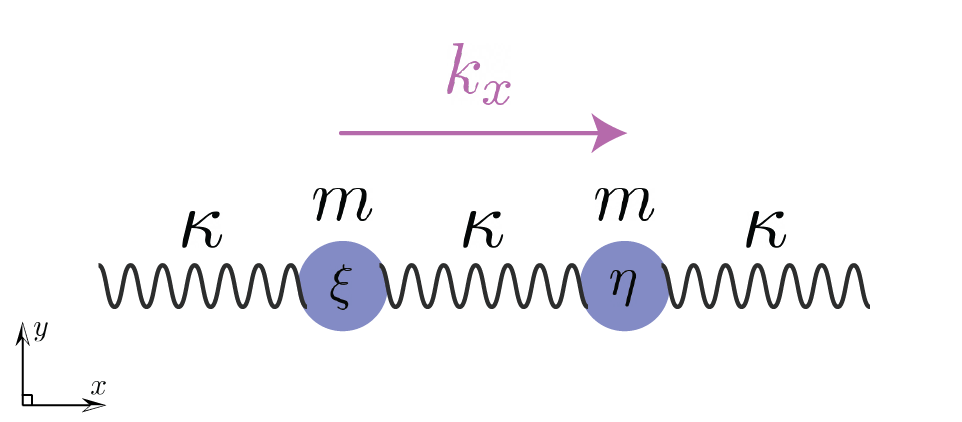
\includegraphics[width=.8\linewidth]{1d.png}
  \caption{1a}
  \label{fig:1d}
\end{subfigure}\\
\begin{subfigure}{\textwidth}
  \centering
  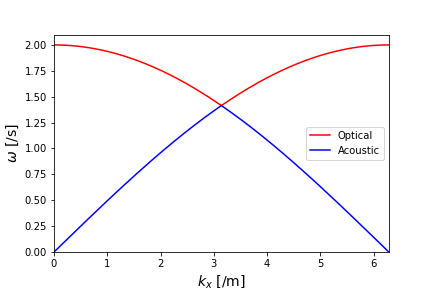
\includegraphics[width=.8\linewidth]{1d-dispersion.png}
  \caption{1b}
  \label{fig:1d-dispersion}
\end{subfigure}\\
\begin{subfigure}{.3\textwidth}
  \centering
  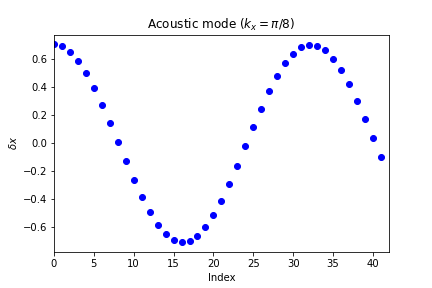
\includegraphics[width=.8\linewidth]{1d-acoustic.png}
  \caption{1c}
  \label{fig:1d-acoustic}
\end{subfigure}
\begin{subfigure}{.3\textwidth}
  \centering
  \includegraphics[width=.8\linewidth]{1d-light.png}
  \caption{1d}
  \label{fig:1d-light}
\end{subfigure}
\caption{plots of....}
\label{fig:fig}
\end{figure}

Before breaking TRS by introducing Coriolis force on the non-inertial reference frame, we want to check how the system works on the inertial frame of reference for comparison.

\begin{align}
m\ddot\xi^n &= -2k\xi^n + k\eta^n + k\eta^{n-1}\\
\ddot\xi^n &= \frac{k}{m}(-2\xi^n + \eta^n + \eta^{n-1})\\
-\omega^2\xi^n &= \omega_0^2(-2\xi^n + \eta^n + \eta^{n-1})
\end{align}

with

\begin{align}
\xi &= C e^{i\omega t}\\
\omega_0^2 &= \frac{k}{m}
\end{align}

By repeating same process on $\eta$ we can get the following result.

\begin{align}
-\omega^2\eta^n &= \omega_0^2(-2\eta^n + \xi^n + \xi^{n-1})
\end{align}


and by defining bloch's constant with $K = e^{ik}$

$$
K = e^{ik}
$$


\subsubsection{Exact model}

We don't need to use exact model like fig because wavenumber propagates
through tangential direction does not have measurable effect on
overall dispersion relation.

\subsection{1D mechanical lattice on non-inertial reference frame}

\subsubsection{With coriolis force}

\subsubsection{With coriolis force and centrifugal force}

\subsection{2D mechanical graphene on inertial frame of reference}

\subsection{2D mechanical graphene on non-inertial reference frame}

\subsubsection{With coriolis force}

\subsubsection{With coriolis force and centrifugal force}

\end{document}